%!TEX root = ../Hardtung_PP_WiSe1920.tex

\section{Introduction}
\label{sec:introduction}

Origami is the Japanese art of folding paper into models of animals, people or other objects. Creating instructions for folding these \gls{origami} models is a tedious and time consuming task. These so called origami diagrams (see Figure \ref{fig:craneDiagram}) have to be accurate representations of the paper for every folding step, in order to unambiguously explain how to fold the model. Every flap, crease and edge has to be drawn (see Section \ref{sec:generalRules} for exceptions), which makes the process slow and especially error-prone for complex models. While the crane model in Figure \ref{fig:craneDiagram} can be folded in 17 steps more complex models can take hundreds of steps to complete.\\
\begin{figure}[htbp]
	\centering
	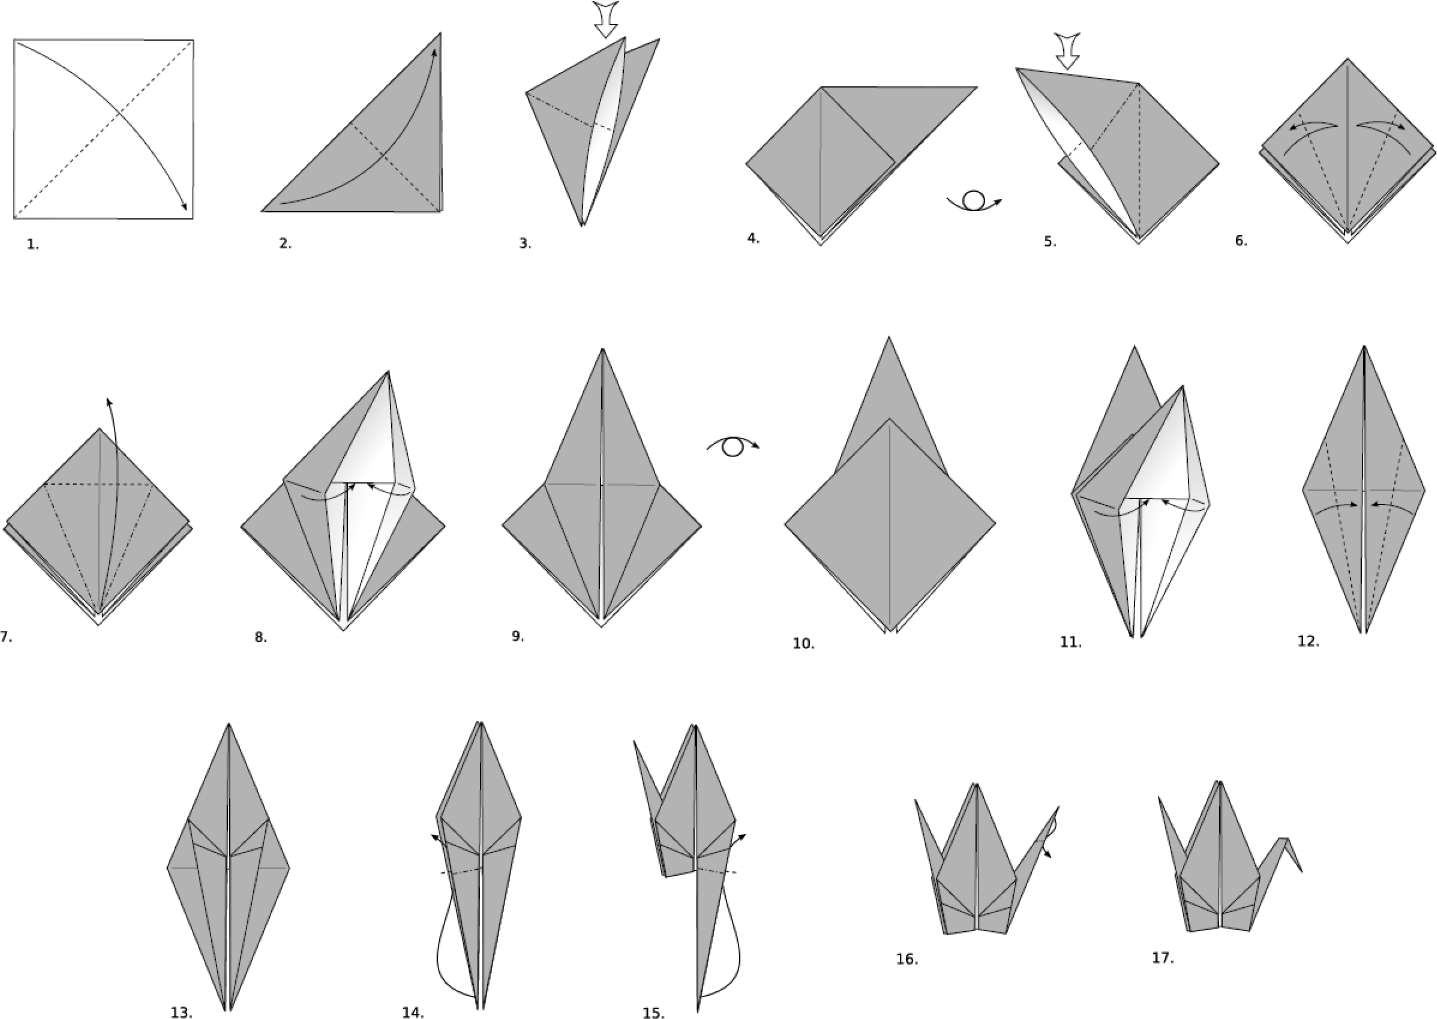
\includegraphics[width=0.6\textwidth]{Crane}
	\caption[Crane Diagram]{Crane Diagram - [Andrew Hudson 2011 \cite{Hudson}]}
	\label{fig:craneDiagram}
\end{figure}\\
Historically, diagrams got either drawn by hand or created with the help of digital vector programs like Inkscape \footnote{\url{https://inkscape.org/}} or Adobe Illustrator \footnote{\url{https://www.adobe.com/de/products/illustrator.html}}. Even though the digital diagramming improved the accuracy of the finished instructions, the task itself was still quite time consuming especially for models with hundreds of steps.\\
In contrast to diagramming programs there have been several attempts at creating programs that virtually fold the paper in order to create models. These include amongst others eGami by Jack Fastag \cite{eGami}, Origami Simulation by Robert J. Lang \cite{origamiSimulation} and the Foldinator Project by John Szinger \cite{foldinator}. However none of these projects ever got outside the prototype phase and they haven't been updated in years.\\
Up until the point of this publication there is no publicly available program that offers specific features for the origami diagramming process.  The previously mentioned vector programs can be used for diagramming, however as they weren't developed with origami diagramming in mind, there are a lot of shortcomings in their feature set. These shortcomings of current programs will be further elaborated on in Section \ref{sec:requirementAnalysis}.\\
The goal for this project is to develop a desktop application that implements features specifically for the origami diagramming process. The standardized symbols and overall notations have to be included and the program has to offer functions that increase the efficiency of creating diagrams.\\
This work starts with an overview and subsequently a categorization of current origami diagramming notations. Based on these findings, a requirements analysis can be carried out in order to define the required features of the planned program. Any problems or other findings during the development process will be documented so that they may be beneficial to others in the future.

